\documentclass[11pt, a4paper, twocolumn]{jsarticle}

\makeatletter

%%% 個人設定 
\usepackage{amsmath,amssymb}
\usepackage{amsthm}
\usepackage{graphicx}
\usepackage[paperheight={29.7truecm},paperwidth={21truecm},hmargin={24.8truemm,24.8truemm},vmargin={30truemm,30truemm}]{geometry}

\bibliographystyle{plain}

\newcommand{\R}{\mathbf R}
\newcommand{\N}{\mathbf N}
\newcommand{\Q}{\mathbf Q}
\newcommand{\Z}{\mathbf Z}
\newcommand{\T}{\{0\}^*}
\newcommand{\D}{D}
\newcommand{\classP}{\mathbf{P}}
\newcommand{\classPSPACE}{\mathbf{PSPACE}}
\newcommand{\classNP}{\mathbf{NP}}
\newcommand{\classPH}{\mathbf{PH}}
\newcommand{\classPP}{\mathbf{PP}}
\newcommand{\classCH}{\mathbf{CH}}
\newcommand{\C}{\mathbf{C}}

\theoremstyle{definition}
\newtheorem{theorem}{定理}[section]
\newtheorem{lemma}[theorem]{補題}
\newtheorem{collorary}[theorem]{系}
\newtheorem{definition}[theorem]{定義}
\newtheorem{hypothesis}[theorem]{仮定}

\renewcommand{\proofname}{\bf 証明} 

%%% \proc != 0 ならば証明などをとばす.
\newcommand{\proc}{1}


%%% 数式中の大文字ギリシャ文字を斜体化
\renewcommand{\Lambda}{\varLambda}
\renewcommand{\Gamma}{\varGamma}

%%% (i), (ii), (iii), (iv)
\def\theenumi{\roman{enumi}}
\def\labelenumi{(\theenumi)}

%%% 数式番号を(章.num) に
\renewcommand{\theequation}{\thesection.\arabic{equation}}
\@addtoreset{equation}{section}

%%% 表番号を 章.num に
\renewcommand{\thetable}{\thesection.\arabic{table}}
\@addtoreset{table}{section}

%%% 図番号を 章.num に
\renewcommand{\thefigure}{\thesection.\arabic{figure}}
\@addtoreset{figure}{section}

%%% align* などで指定した場所だけ数式番号を置く
\newcommand{\taghere}{{
\stepcounter{equation}
\tag{\theequation}
}}

\makeatother

\title{滑らかな常微分方程式の計算量}

\author{%
太田浩行\thanks{東京大学, \texttt{hota@is.s.u-tokyo.ac.jp}} 
\and
河村彰星\thanks{東京大学}%
\and
マルチン・ツィーグラー\thanks{Martin Ziegler, ダルムシュタット工科大学}
\and
カルステン・レースニク\thanks{Carsten R\"osnick, ダルムシュタット工科大学}
}
%\和暦
\date{}

\begin{document}

\maketitle

%%% 以下に,予稿の本文を記述して下さい.

\begin{abstract}
The computational complexity of the solution~$h$ to 
the ordinary differential equation 
$h(0)=0$, $h'(t) = g(t, h(t))$ 
under various assumptions on the function $g$
has been investigated
in hope of understanding the intrinsic hardness of 
solving the equation numerically. 
Kawamura showed in 2010 that the solution~$h$ can be $\classPSPACE$-hard
even if $g$ is assumed to be Lipschitz continuous. 
We place further requirements on the smoothness of $g$ 
and obtain the following results: 
the solution~$h$ is still $\classPSPACE$-hard
if $g$ is assumed to be continuously differentiable; 
for each $k \geq 2$, 
the solution~$h$ is hard for the counting hierarchy 
if $g$ is assumed to be $k$-times continuously differentiable. 
\end{abstract}


\section{序論}

\emph{計算可能解析学} (Computable Analysis) \cite{weihrauch00:_comput_analy} では
計算可能性理論や計算量理論の視点から解析学を扱う. 
「計算可能な実数」や「多項式時間計算可能な実関数」といった概念を定義し
(本稿では\ref{section: preliminaries}節で説明する), 
解析学に現れる様々な実数や実関数の本質的な難しさを分析する. 

連続実関数 $g \colon [0,1] \times \R \to \R$ に対して次の常微分方程式を考える. 
\begin{align}
 \label{eq:ode}
 h(0) & = 0, &
 \D h(t) & = g(t,h(t)) \quad (t \in [0,1])
\end{align}
ただし $\D h$ は $h$ の導関数.
本稿では $g$ が多項式時間計算可能であるとき, 
解 $h$ がどれほど複雑でありうるかを考える.

$g$ に多項式時間計算可能であることの他に何の制限も設けない場合, 
解 $h$ (一般に一意でない) は計算不能でありうるため,
様々な制限のもと $h$ の計算量が研究されている (表 \ref{table:related}).
この表では下に向うにつれて左列の条件が強まっており, 
$g$が(大域的) Lipschitz条件を満たせば解$h$が一意であるが, 
表の第3行にある通りこのとき唯一解$h$は
ちょうど$\classPSPACE$困難でありうることがわかっている\cite{kawamura2010lipschitz}. 
本稿の目的はより強く$g$に滑らかさの仮定を置いたときの
$h$の複雑さを調べることである. 

\begin{table}
\renewcommand\arraystretch{1.3}
\begin{center}
 \caption{多項式時間計算可能実関数 $g$ の常微分方程式 (\ref{eq:ode}) の解 $h$ の計算量}
 \label{table:related}
 \begin{tabular}{lll}
  制限 & 上界 & 下界 \\
  \hline
   --- & --- & 計算不可能たりうる \cite{pour1979computable} \\
  $h$ が $g$ の唯一解 & 計算可能 \cite{coddington1955theory}
  & 任意の時間がかかりうる \cite{ko1983computational, miller1970recursive} \\
  $g$ が Lipschitz 条件を満たす & 多項式領域計算可能 \cite{ko1983computational}
      &	$\classPSPACE$ 困難になりうる \cite{kawamura2010lipschitz}\\
  $g$ が $(\infty, 1)$ 回連続微分可能 & 多項式領域計算可能 & \parbox[t]{14zw}{$\classPSPACE$ 困難になりうる\\{}[本稿定理\ref{DifferentiableIsPspace}]} \\
  $g$ が $(\infty, k)$ 回連続微分可能 & 多項式領域計算可能 & \parbox[t]{14zw}{$\classCH$ 困難たりうる\\{}[本稿定理\ref{KTimesIsCH}]} \\
  $g$ が解析的 
  & 多項式時間計算可能 \cite{ko1988computing, kawamura2010complexity} 
  & ---
 \end{tabular}
\end{center}
\end{table}

% 一方で $g$ が解析的であるとき, 解 $h$ も解析的となり, 
% このとき $h$ は多項式時間計算可能である.
% そこで本稿ではこの隔たりを埋めるため, 滑らか
% つまり微分可能な実関数 $g$ について $h$ の計算量がどれほどになりうるかを調べた.

一般に数値計算においてはしばしば, 
或る種の算法を適用できるようにするため, 
或いは解析しやすくするために, 
与えられる関数に何らかの滑らかさ (十分な回数微分可能であるなど) を仮定すると
都合のよいことがある. 
しかしこれは経験則にすぎず, 
実際に滑らかさの仮定が
解の複雑さを計算量の意味で抑える効果をもつのかについては
あまり論ぜられて来なかった. 

本稿で扱う微分方程式についていえば, 
極端なのは$g$が解析的である場合であり, 
このときにはテイラー級数として解く議論により, 
表の最下列にあるように$h$は$g$と同じく多項式時間計算可能になる. 
本稿ではLipschitz条件より強いが解析的よりは弱い滑らかさの仮定を考える
(表の第4, 5行). 
ここで$(i, j)$回連続微分可能とは, 
第一, 第二変数についてそれぞれ$i$回, $j$回微分でき, 
その導関数が連続であることである (\ref{section: preliminaries}節).

例えば, 積分の計算量については
無限回微分可能な関数の積分も一般の関数の積分と同等に多項式領域困難であるが,
解析的な関数の積分においては, 多項式時間計算可能である.
つまり無限回微分可能と解析的という制限の間に大きな隔たりをもつ.
最大化でも同様に, 無限回微分可能な関数の最大化は一般の関数の最大化と同じく
$\classNP$ 困難であるが,
解析的な関数の最大化は多項式時間計算可能である.


無限回微分可能な関数の最大化が一般の関数と同じく$\classNP$困難であること
の証明は葛によって与えられているが, その中には間違いが存在する.
その訂正をするなかで, 同じ手法を常微分方程式にも用いることができないかと考え以下の結果を得た.

 \begin{theorem}
  \label{DifferentiableIsPspace}
  多項式時間計算可能かつ $(\infty, 1)$ 回連続微分可能な
  実関数 $g \colon [0,1] \times [-1,1] \to \R$ であって, 
  常微分方程式\eqref{eq:ode}が
  $\classPSPACE$ 困難な解 $h \colon [0, 1] \to \R$ を持つものが存在する.
 \end{theorem}

 \begin{theorem}
  \label{KTimesIsCH}
  任意の自然数 $k \ge 2$ に対して, 
  多項式時間計算可能かつ $(\infty, k)$ 回連続微分可能な
  実関数 $g \colon [0,1] \times [-1,1] \to \R$ であって, 
  常微分方程式(\ref{eq:ode})が
  $\classCH$ 困難な解 $h \colon [0, 1] \to \R$ を持つものが存在する.
 \end{theorem}

ここで $g \colon [0,1] \times \R \to \R$ でなく
$g \colon [0,1] \times [-1, 1] \to \R$ と書いたのは, 
本稿では実関数の多項式時間計算可能性を, 
定義域が有界閉領域のときにのみ定義するからである. 
このため $h$ が区間 $[-1, 1]$ の外に値を取ることがあると
方程式(\ref{eq:ode})が意味をなさなくなるが, 
定理\ref{DifferentiableIsPspace}において $h$ が解であるというのは, 
任意の $t \in [0, 1]$ について $h (t) \in [-1, 1]$ が満たされることも含めて述べている.
なお両定理とも Lipschitz 条件よりも強い仮定を置いているため, 
そのような $h$ は $g$ に対して, 存在すれば唯一である. 

また二変数関数 $g$ が
$i+j \le k$ を満たす任意の自然数 $i,j$ について
$(i,j)$ 回連続微分可能であることを, 
$g$ が $k$ 回連続微可能であると言うこともある.
定理\ref{DifferentiableIsPspace}で主張される $g$ は, 
$(\infty, 1)$ 回連続微分可能であるから, 
特に $1$ 回連続微分可能である. 


1回微分可能な実関数においては, より弱い条件であるLipschitz条件を満たすときと同じく,
$\classPSPACE$困難であることを示すことができた.
しかし2回以上微分可能な実関数の常微分方程式においては,
$\classPSPACE$に含まれる計算量クラスである$\classCH$に対して困難であること
のみ示された.

$\classCH$は定数回の計数(数え上げ)による計算量クラスである.
積分が $\#\classP$困難であるように,
離散的な計数が実関数では積分に対応する.
常微分方程式は $h(t)$ にたいして
これは1回微分可能という条件のもとでは
入力に対して十分にフィードバックをかけることが可能だったが,
2回微分可能のという制限によってフィードバックが



 また定理 \ref{KTimesIsCH} において
 任意の $k$ に対して $(\infty, k)$ 階微分可能な関数を考えているが,
 一つの関数が任意の $k$ に対して $k$ 階微分であることを求めているわけではない.
 つまり $g$ が無限回微分可能であると制限しているわけではない. 
 無限回微分可能な関数に対する常微分方程式の計算量は今後の課題である.


\section{準備}
\label{section: preliminaries}

\subsection{表記}
自然数の集合を $\N$, 整数の集合を $\Z$, 実数の集合を $\R$, 
有理数の集合を $\Q$, $\T = \{0^n \mid n \in \N\}$ で表す. 

$A \subset \R$ とする. 一変数関数 $f\colon A \to \R$ が $i$ 回微分可能であるとき,
その $i$ 階導関数を $\D{i}f$ と表記する.

二変数関数 $g \colon A \times B \to \R$ が
$(i, j)$ 回連続微分可能であるとき,
第一変数について $i$ 階, 第二変数について $j$ 階の導関数は
その微分の順序によらず等しい \cite{takagi1968analysis}.
その導関数を $\D{i,j}g$ で表す.

実関数 $f \colon A \to \R$ にたいして $|f| = \sup_{x \in A} f(x)$ と書く.

\subsection{実数の名}
 実数は有限な文字列に符号化できない. 
 そこで文字列から文字列への関数に符号化する.
 \begin{definition}[実数の名]
  関数 $\phi \colon \T \to \Z $ が実数 $x \in [0,1]$ の名であるとは,
  $\phi(0^n) = \lfloor x \cdot 2^n \rfloor$ または
  $\phi(0^n) = \lceil x \cdot 2^n \rceil$ を満たすこと.
 \end{definition}
ここで $\lfloor \cdot \rfloor, \lceil \cdot \rceil$ とはそれぞれ
整数への切り捨て関数と
切り上げ関数である.
つまり実質的には実数 $x$ の名は, 
サイズ $n$ の入力を受け取ると, 精度 $n$ 桁の $x$ の
近似値を返す.
以下では$\phi$ の値を二進数で表すことにし, 
$\phi$ を文字列から文字列への関数として扱う. 

\subsection{計算可能実関数, 多項式時間実関数}

実数を受け取り実数を返す関数を
機械が計算するとはどういうことか定義しよう. 
実数自体が関数として符号化されているため, 
それを読み書きする機構として, 
神託チューリング機械 (以下単に機械という) を使う[図 \ref{fig:model-of-function}].

 \begin{figure}
  \label{fig:model-of-function}
  \begin{center}
   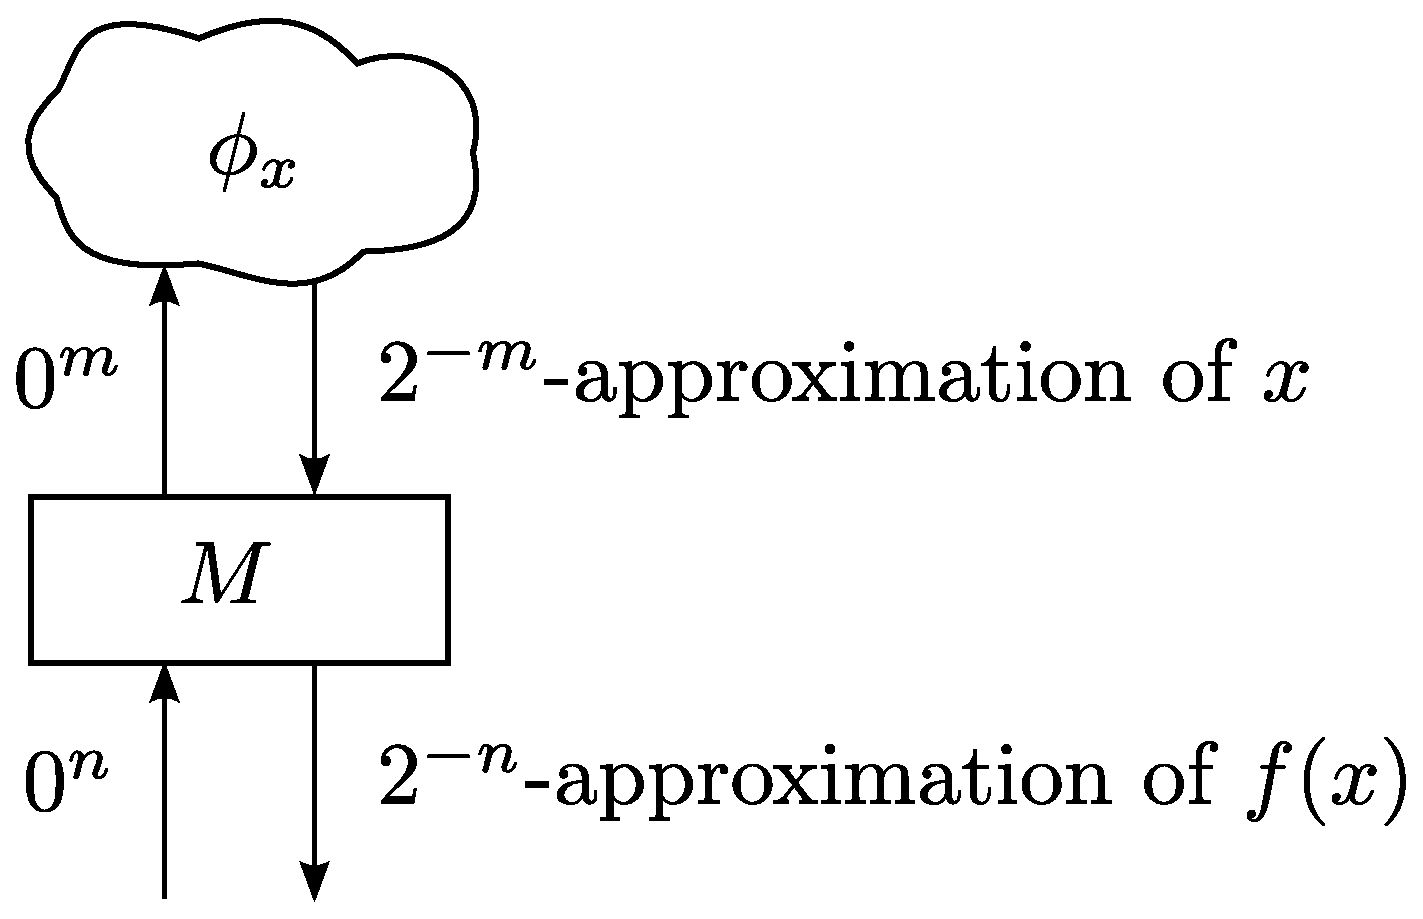
\includegraphics[height=0.15\textheight]{image/model-of-function.eps}
  \end{center}
  \caption{実関数を計算する機械}
 \end{figure}

機械$M$に, 
文字列から文字列への関数$\phi$を神託として与え, 
文字列$0 ^n$を入力として与えたとき, 
出力される文字列を$M ^\phi (0 ^n)$で表す. 
つまり$M ^\phi$をやはり文字列から文字列への関数とみる. 

\begin{definition}
$A$を$\R$の有界閉区間とする. 
神託機械 $M$ が実関数 $f\colon A \to \R$ を計算するとは,
任意の実数 $x \in A$, 任意の $x$ の名 $\phi_x$ にたいして,
$M^{\phi_x}$ が $f(x)$ の名であること.
\end{definition}

$f$が二変数関数であるときには神託を二つ取る機械を考えて同様に定義する. 

 計算可能な実関数は Grzegorczyk によって初めて形式的に定義され,
 \cite{grzegorczyk1955computable}.
 多変数関数のモデルも, 変数と同じ数だけ神託を持つ神託機械によって同様に定義される.

 ある実関数が計算可能であるとは, その関数を計算する神託機械が存在することである.
 同様に, ある実関数が多項式時間計算可能であるとは, その関数を計算する多項式時間神託機械が存在することである.

 神託機械 $M$ がある実関数族 $(f_u)_u$ を計算するとは,
 入力 $u$ を受けったとき, $M_u$ が $f_u$ を計算することである.
 実関数族が多項式時間計算可能であるとは, その実関数族を計算する
 多項式時間神託機械が存在することである.
 

 神託機械 $M$ で $f$ を計算するとき, 求める精度 $n$ にたいして,
 $x$ の近似値に必要な精度 $m$ が定まるため,
 計算可能な関数は連続である.
 また $n$ と $m$ の対応関係と有理数における近似値を与えることで,
 計算可能実関数や多項式時間計算可能実関数にたいして,
 神託機械を用いない同値な特徴付けが可能である.

 \begin{lemma}
  \label{lem:type1representation}
  実関数 $f\colon [0,1] \to \R$ にたいして,
  $\phi_f\colon (\Q \cap [0, 1]) \times \T \to \Q$, $m_f\colon \N \to \N$は
  \begin{align}
   |\phi_f(d, 0^n) - f(d)| \le 2^{-n} 
   &\qquad (d \in (\Q \cap [0,1]), \quad n \in \N)\\
   |x-y| \le 2^{-p_f(m)} \Rightarrow |f(x) - f(y)| \le 2^{-m}
   &\qquad (x, y \in [0, 1], \quad m \in \N)
  \end{align}
 をみたす関数とする.
  \begin{itemize}
   \item $f$ が計算可能であることは, 計算可能な $\phi_f, m_f$ が存在することと同値である. 
   \item $f$ が多項式時間計算可能であることは, 多項式時間計算可能な 
  $\phi_f$, 多項式 $m_f$ が存在することと同値である.
  \end{itemize} 
\end{lemma}

\subsection{困難性}

 関数の下限を示すために, 実関数の計算量クラスに対する困難性を定義する.

 まず実関数の言語に対する還元を定義する.
 言語 $L$ が実関数 $f\colon [0,1] \to \R$ に多項式時間還元可能であるとは,
 $f$ を計算する機械を使って $L(u)$ を多項式時間で計算可能であることである.
 つまり $f$ を計算する機械が与えられ, 入力 $u$ にたいして,
 精度 $n$ を $f$ に与え, ある実数 $x_u$ の神託を模倣し, $f(x_u)$ の $n$ 桁近似値から,
 $u$ が $L$ に含まれるか否かを多項式時間で計算可能であることである
 [図 \ref{fig:reduction}].
 厳密には以下のように定義する.

 \begin{definition}[多項式時間還元可能]
  言語 $L$ が実関数 $f\colon [0,1] \to \R$ に多項式時間還元可能であるとは, 
  任意の文字列 $u$ にたいして, 以下を満たす実数 $x_u \in [0,1]$
  多項式時間計算可能な関数 $R,S,T$ が存在すること.
  \begin{itemize}
   \item $R\colon N \times N \to \{0,1\}, \quad S\colon \N\times \T \to \N, \quad
  T\colon \N \to \T$;
   \item $S(u, \cdot)$ は実数 $x_u$ の名;
   \item 任意の $f(x_u)$ の名 $\phi$ にたいして
	 \[
	  L(u) = R(u, \phi(T(u))).
	 \]
  \end{itemize}
 \end{definition}
 以下単に言語が実関数に還元可能といった場合, 多項式時間還元可能をしめす.
 計算量 $C$ にたいして, 関数 $f$ が $C$困難であるとは,
 任意の $C$ に含まれる言語が $f$ に還元可能であることと定義する.

 \begin{figure}
  \begin{center}
  \label{fig:reduction}
  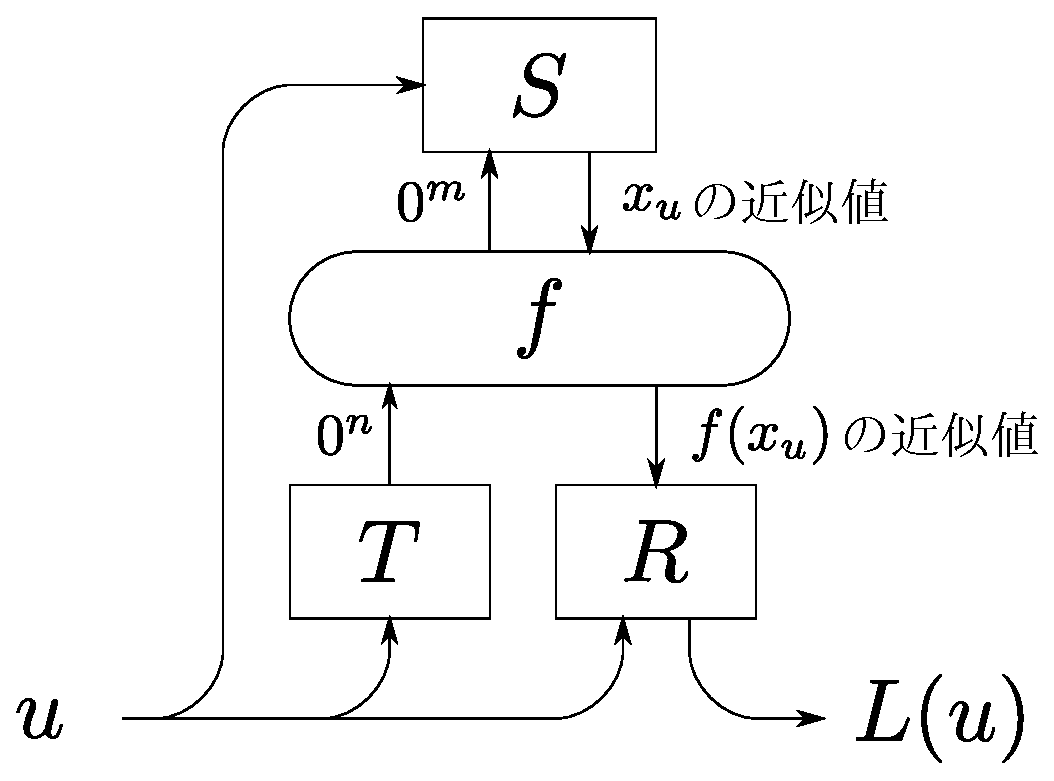
\includegraphics[height=0.2\textheight]{image/reduction.eps}
  \caption{言語 $L$ から関数 $f$ への還元}
  \end{center}
 \end{figure}

 

\section{1回連続微分可能関数と常微分方程式}
\label{section:differentiable}

この節では定理 \ref{DifferentiableIsPspace},
つまり$(\infty, 1)$階連続微分可能な関数の常微分方程式の解は
\PSPACE 困難でありうることを示す.
\ifnum \proc = 1
ただし紙面の都合上, 詳細な証明は省き, 証明の概略を述べるに止める.
\fi

証明の流れとして, まず補題 \ref{WeakFeedback} によりの
$L \in \PSPACE$ を認識する関数族$(G_u)_u, (H_u)_u$ を得る.
そして $(G_u)_u, (H_u)_u$ を模倣する
実関数族 $(g_u)_u, (h_u)_u$ を構成し(補題 \ref{DifferentiableFamily}),
$(g_u)_u, (h_u)_u$ から定理 \ref{DifferentiableIsPspace} で求める $g, h$を構成する.


\subsection{多項式段一様関数族の差分方程式と\PSPACE}


任意の言語 $L \in \PSPACE$ について, 
その差分方程式が $L$ を認識する
多項式段一様な関数族 $(G_u)_u$ が存在すること(補題 \ref{WeakFeedback})は
河村によって示されているがその証明の概略を示す.

\PSPACE 完全な言語である
\textsf{QBF} を認識する $(G_u)_u$ を構成することにより,
任意の $L \in \PSPACE$ を認識する多項式段一様な関数族 $(G_u)_u$ が存在することを示す.
ここで \textsf{QBF} とは,
文字列 $u$ を $\psi = Q_1 x_1 \cdots Q_n x_n \phi(x_1, \dots, x_n)$ と解釈したとき 
$u \in \textsf{QBF} \Leftrightarrow \psi = T$ によって定義される言語である. 
ただし$Q_i$ は$\exists$ または $\forall$,  
$\phi(x_1, \dots, x_n)$ は $x_i$ 以外の変数を含まない論理式とする. 

論理式 $\psi = Q_1 x_1 \cdots Q_n x_n \phi(x_1, \dots, x_n)$ の値を
$\vee, \wedge$によってラベル付された二分木によって計算することを考える. 
量化子$Q_1 x_1$ を除き $x_1$ を $T$ と $F$ に置き換えた式をそれぞれ
$\psi_T = Q_2 x_2 \cdots Q_n x_n \phi(T, x_2, \dots, x_n)$,
$\psi_F = Q_2 x_2 \cdots Q_n x_n \phi(F, x_2, \dots, x_n)$ と置くと
$Q_1=\forall$ ならば $\psi = \psi_T \wedge \psi_F$, 
$Q_1=\exists$ ならば $\psi = \psi_T \vee \psi_F$.
つまり変数の1つ少ない2つの論理式と量化子によってもとの論理式の値も決まる.
これを再帰的に繰り返すことで $\psi$ は計算可能であり, 
それは深さ $n$ の二分木を葉から根へ値を定めていくことと同じである.
この過程は二分木の深さが段数に, 幅が列数に対応する形で
多項式段一様な関数による差分方程式で模倣可能であるため,
\textsf{QBF} を認識する多項式段一様関数の差分方程式が存在する.



\subsection{多項式段差分方程式を模倣する関数族}


\begin{lemma}
 \label{DifferentiableFamily}
 任意の言語 $L \in $ \PSPACE に対して, 
 係数のみに $i$ を含む多項式 $\mu_i$ が存在して,
 任意の多項式 $\gamma$ に対して,
 多項式 $\rho$, 関数族 $(g_u)_u, (h_u)_u$ で, 
 $(g_u)_u$ は多項式時間計算可能であり,
 各二進文字列 $u$ に対して以下を満たすものが存在する.
 \begin{enumerate}
  \item $g_u\colon [0,1] \times [-1,1]\to \R, \quad h_u\colon [0,1] \to [-1,1]$;
  \item $h_u$ は $g_u$ の常微分方程式 (\ref{eq:ode}) の解; 
  \item $g_u$ は $(\infty, 1)$ 階連続微分可能;
  \item 任意の $i \in \N$, $y \in [-1,1]$ に対して
	\begin{equation*}
	 \D{i, 0} g_u(0,y) = \D{i, 0} g_u(1,y) = 0;
	\end{equation*}
  \item \label{enum:infty1}
	任意の $i \in \N$ に対して
	\begin{align*}
	 |\D{i,1} g_u| &\leq 2^{\mu_i (|u|) - \gamma(|u|)}, &
	 |\D{i,0} g_u| &\leq 2^{\mu_i (|u|) - \gamma(|u|)};
	\end{align*}
  \item $h_u(1) = 2^{-\rho(|u|)}L(u)$.
 \end{enumerate}
\end{lemma}

 この補題より関数族 $(g_u)_u, (h_u)_u$ で $h_u$ は $g_u$ の常微分方程式の解であり,
 $g_u$は滑らかであり, 各 $h_u(1)$ に $L(u)$ の情報を持つものの存在が示される.
 条件 (iii) -- (v) はすべて定理 \ref{DifferentiableIsPspace} の $g$ を
 滑らかな関数とするために必要となる条件である.
 詳細については定理の証明の際に説明する.
 

 この補題の証明の基本的な流れを説明する.
 任意の言語 $L \in \PSPACE$ に対し, 
 補題 \ref{WeakFeedback} を用いて $L$ を認識する $(G_u)_u$ 
 及びその差分方程式の解 $(H_u)_u$ を得る.
 各 $G_u, H_u$ を模倣する
 $(\infty, 1)$階連続微分可能な $g_u \colon [0,1] \times [-1, 1] \to \R$ 
 とその常微分方程式の解 $h_u \colon [0,1] \to \R$ を構成する.
 また $(G_u)_u$ の一様性から $(g_u)_u$ の多項式時間計算可能性を示す.


 上記の証明は基本的に, リプシッツ連続条件の場合の証明と変わらない.
 違いは $g_u$ を滑らかな関数にするため, 
 以下のような滑らかな多項式時間実関数 $f \colon [0,1] \to \R$ を用いて
 $g_u$ を構成している点である.

 \begin{lemma}[補題 3.6. \cite{ko1991complexity}]
  \label{SmoothFunction}
  以下を満たす多項式時間無限回微分可能実関数 $f \colon [0,1] \to \R$ が存在する.
  \begin{enumerate}
   \item $f(0) = 0, \quad f(1) = 1$;
   \item 任意の $n \ge 1$ で $f^{(n)}(0) = f^{(n)}(1) = 0$;
   \item $f$ は $[0,1]$ で単調増加;
   \item 任意の $n \ge 1$ で $f^{(n)}$ は多項式時間実関数.
  \end{enumerate}
 \end{lemma} 


%%% 証明は削除, 残っているバージョン tag:proof


\subsection{定理 \ref{DifferentiableIsPspace} の証明}

 \PSPACE 完全な言語 {\sf QBF} 補題 \ref{DifferentiableFamily} から得られる
 $(g_u)_u$ と $(h_u)_u$ から滑らかな $g$ と
 その常微分方程式の解で \PSPACE 困難な $h$ を構成する.
 各 $h_u(1)$ には $L(u)$ の情報が含まれるため,
 すべての $h_u$ を一つの関数 $h$ に埋め込みたい.
 そこで [0,1] を無限の区間に分割し, $h$ の各文字列 $u$ に対応する区間
 $[l^-_u, c_u]$ に $h_u$ を
 縮小して埋め込む. 
 ただし次の文字列 $u'$ の計算に影響を与えないために,
 $h_u$ を定義域方向について反転したものを
 区間 $[c_u, l^+_u]$ に埋め込むことで影響を相殺する.
 つまり $h(l^-_u) = 0,\ h(c_u) = 2^{-\rho'(|u|)} L(u),\ h(l^+_u) = 0$ を満たす
 ように $h_u(t)$埋め込む.
 ただし $\rho'$ とは $\rho$ に縮小率をかけたものとする.
 同様に $g$ は $h$ が常微分方程式の解となるよう,
 各文字列 $u$ に対応する区間に $g_u$ を縮小して埋め込む.

 リプシッツ連続条件の場合と異なる点は, $g_u$ を構成する時点で
 $(\infty, 1)$ 階連続微分可能にするために,
 $|\D{i,0} g_u|, |\D{i,0} g_u|$ の大きさを制限する点である
 (補題 \ref{DifferentiableFamily} の (\ref{enum:infty1})).
 

%%% 証明は削除, 残っているバージョン tag:proof


\section*{謝辞}

本研究を遂行し発表するにあたり
日本学術振興会「組織的な若手研究者等海外派遣プログラム」及び
文部科学省科学研究費補助金若手研究(B)\,23700009による援助を受けた. 
記して謝意を表する. 


\begin{thebibliography}{10}
\narrowbaselines

\bibitem{coddington1955theory}
E.A.~Coddington and N.~Levinson.
\newblock {\em Theory of Ordinary Differential Equations}.
\newblock McGraw-Hill, 1955.

\bibitem{grzegorczyk1955computable}
A.~Grzegorczyk.
\newblock Computable functionals.
\newblock {\em Fund. Math}, 42(19553):168--202, 1955.

\bibitem{kawamura2010complexity}
A.~Kawamura.
\newblock Complexity of initial value problems.
\newblock To appear in {\em Fields Institute Communications}.

\bibitem{kawamura2010lipschitz}
A.~Kawamura.
\newblock Lipschitz continuous ordinary differential equations are
  polynomial-space complete.
\newblock {\em Computational Complexity}, 19(2):305--332, 2010.

\bibitem{kawamura2010operators}
A.~Kawamura and S.~Cook.
\newblock Complexity theory for operators in analysis.
\newblock In {\em Proceedings of the 42nd ACM Symposium on Theory of
  Computing}, pages 495--502, 2010.

\bibitem{ko1983computational}
K.I. Ko.
\newblock On the computational complexity of ordinary differential equations.
\newblock {\em Information and Control}, 58(1-3):157--194, 1983.

\bibitem{ko1991complexity}
K.I. Ko.
\newblock {\em Complexity Theory of Real Functions}.
\newblock Birkh{\"a}user Boston, 1991.

\bibitem{ko1988computing}
K.I. Ko and H.~Friedman.
\newblock Computing power series in polynomial time.
\newblock {\em Advances in Applied Mathematics}, 9(1):40--50, 1988.

\bibitem{miller1970recursive}
W.~Miller.
\newblock Recursive function theory and numerical analysis.
\newblock {\em Journal of Computer and System Sciences}, 4(5):465--472, 1970.

\bibitem{pour1979computable}
M.B. Pour-el and I.~Richards.
\newblock A computable ordinary differential equation which possesses no
  computable solution.
\newblock {\em Annals of Mathematical Logic}, 17(1-2):61--90, 1979.

\bibitem{weihrauch00:_comput_analy}
K. Weihrauch.
\newblock {\em Computable Analysis: An Introduction}.
\newblock Texts in Theoretical Computer Science. Springer, 2000.

\bibitem{takagi1968analysis}
高木貞治.
\newblock {\em 解析概論}.
\newblock 岩波書店, 1968.

\end{thebibliography}

\end{document}
